%% German Document Type Classification using CNNs — Phase III report
%% Built on the course SS26 Machine Learning elsarticle template.
%% Overleaf: New Project -> Upload Project with this folder (main.tex,
%% Bibliography.bib, figures/). Compiler: pdfLaTeX. elsarticle is built in.
%%
%% TEMPLATE RULE: the instructor asks you to keep the template guidance text
%% (commented out) and write your content beneath it. The verbose guidance has
%% been condensed into short % reminders here; paste back the full guidance from
%% elsarticle-template-num.tex if your instructor requires every line preserved.
\documentclass[preprint,12pt]{elsarticle}

\usepackage{amssymb}
\usepackage{amsmath}
\usepackage{lineno}
\usepackage{xcolor}
\usepackage{array}
\usepackage{multirow}
\usepackage{pifont}
\usepackage{adjustbox}
\usepackage{booktabs}
\usepackage{rotating}
\usepackage{colortbl}
\usepackage{tabularx}
\usepackage{makecell}
\usepackage{threeparttable}
\usepackage{graphicx}
\usepackage{subcaption}
\usepackage{url}

\newcommand{\cmark}{\ding{51}} % yes
\newcommand{\xmark}{\ding{55}} % no
\newcommand{\pmark}{\textcolor{orange}{$\sim$}} % partial

\journal{Pattern Recognition (Course Project, SS26)}

\begin{document}

\begin{frontmatter}

%%%%%%%%%%%%%%%%%%%%%%% Title %%%%%%%%%%%%%%%%%%%%%%%
% Title should identify the practical problem, the image task, the modelling
% approach, and the application domain.
\title{An Explainable Transfer-Learning Framework for German Document-Type
Classification from Scanned Page Layout}

%%%%%%%%%%%%%%%%%%%%%%% Author Details %%%%%%%%%%%%%%%%%%%%%%%
\author[label1]{Ashok Kumar Meena}
\affiliation[label1]{organization={Department of Software Engineering, University of Europe for Applied Sciences},
            addressline={Think Campus, Konrad-Zuse-Ring 11},
            city={Potsdam},
            postcode={14469},
            state={Brandenburg},
            country={Germany}}

%%%%%%%%%%%%%%%%%%%%%%% Abstract %%%%%%%%%%%%%%%%%%%%%%%
\begin{abstract}
German-speaking archives, regulators, and tender portals digitise millions of
scanned pages every year, and the first step of every routing workflow is
deciding what kind of document each page is.
Manual routing is slow and costly, while text-based pipelines depend on
fragile optical character recognition over mixed German fonts and poor scans.
Prior document-image research is dominated by English benchmarks, and there is
little work that classifies German pages from visual layout alone while also
explaining and stress-testing the model.
This study builds and rigorously evaluates a convolutional neural network (CNN)
framework that classifies scanned German document pages into six DocLayNet
categories using only the visual page layout, comparing a custom CNN trained
from scratch against an ImageNet-pretrained ResNet50 fine-tuned in two stages.
Models are evaluated with accuracy, macro precision, recall, and F1, one-vs-rest
ROC and AUC, confusion matrices, Grad-CAM attention maps, and a phone-camera
robustness test.
On the held-out DocLayNet-base test split, ResNet50 reaches 0.761 accuracy,
0.724 macro-F1, and 0.956 macro-AUC, decisively outperforming the from-scratch
CNN, which collapses toward the majority class (0.082 macro-F1, 0.479 macro-AUC).
ResNet50 loses only about 0.118 macro-F1 under simulated phone-camera
degradation, and Grad-CAM confirms that it attends to mastheads and structural
page regions.
The best model is deployed as a public web service, demonstrating an
end-to-end, reproducible, and explainable pipeline for German document routing.
\end{abstract}

%%%%%%%%%%%%%%%%%%%%%%% Graphical Abstract %%%%%%%%%%%%%%%%%%%%%%%
% TODO(student): provide one publication-quality summary figure (problem ->
% dataset -> preprocessing -> custom CNN + ResNet50 -> evaluation -> Grad-CAM ->
% deployment). Make it in PowerPoint/Canva and export as PDF, then uncomment.
\begin{graphicalabstract}
%\includegraphics{figures/graphical_abstract.pdf}
\end{graphicalabstract}

%%%%%%%%%%%%%%%%%%%%%%% Research Highlights %%%%%%%%%%%%%%%%%%%%%%%
\begin{highlights}
\item Classifies scanned German document pages into six types from layout alone, without OCR.
\item Custom CNN vs.\ ImageNet-pretrained, two-stage fine-tuned ResNet50 on DocLayNet.
\item ResNet50 attains 0.761 accuracy, 0.724 macro-F1, and 0.956 macro-AUC on the test split.
\item Grad-CAM shows the model attends to mastheads and structural page regions.
\item Robust to phone-camera degradation and deployed as a public web service.
\end{highlights}

%%%%%%%%%%%%%%%%%%%%%%% Keywords %%%%%%%%%%%%%%%%%%%%%%%
\begin{keyword}
Document image classification \sep Convolutional neural networks \sep
Transfer learning \sep ResNet50 \sep Explainable AI (Grad-CAM) \sep DocLayNet
\end{keyword}

\end{frontmatter}

\linenumbers

%==================================================================
\section{Introduction}
% The introduction establishes the practical problem, why CNNs fit, the gap, and
% the study's contributions.

\subsection{Application Background and Practical Importance}
Document classification is a foundational step in the digitisation pipelines of
administrative, legal, scientific, and financial archives.
German-speaking institutions such as the Deutsche Digitale Bibliothek, the
Bundesarchiv, EU tender portals, and federal regulatory bodies process millions
of scanned pages every year.
Once a page is scanned, the first downstream decision is almost always
``what kind of document is this?'', because routing an invoice differs from
routing a patent, which differs again from routing a regulatory notice.
Performing this triage manually is slow, expensive, and error-prone, and it does
not scale to the volume of incoming material.
Incorrect or delayed routing propagates errors into every later stage, from
indexing and retrieval to compliance and archival.
Automated image-based classification can absorb this triage at scale and free
human experts for higher-value tasks.
The economic and administrative pressure to automate makes document-type
classification an ideal target for machine learning.

\subsection{Machine Learning and Computer Vision Context}
Image-based machine learning learns discriminative visual features directly from
pixels rather than from hand-crafted rules.
Convolutional neural networks (CNNs) are particularly suited to documents
because their convolutional filters capture local layout patterns such as
headers, columns, tables, and whitespace, and pooling layers aggregate them into
global structure~\cite{he2016deep}.
Unlike text pipelines, a layout-based CNN does not depend on accurate optical
character recognition and is therefore robust to scan noise and font variety.
This is important for German documents, whose long compound words alter
line-wrapping and whose official mastheads differ markedly from English layouts.
Manual feature engineering cannot easily encode these cues, whereas a CNN learns
them from data.
The main practical challenge is the limited amount of labelled German document
imagery available for training.

\subsection{Transfer Learning for the Selected Problem}
Training a deep CNN from random initialisation typically requires very large
labelled datasets, which are unavailable for German document images.
Transfer learning addresses this by reusing low-level visual features learned on
large natural-image corpora such as ImageNet~\cite{deng2009imagenet,russakovsky2015imagenet}.
A pretrained backbone such as ResNet50~\cite{he2016deep} already encodes edges,
textures, and shapes that transfer to page structure, so only a small classifier
head must be learned from scratch.
Fine-tuning the final residual block then adapts these features to the document
domain without destroying them~\cite{weiss2016survey}.
This study compares such a transfer-learning model against a custom CNN baseline
to quantify exactly how much pretraining helps on a small, imbalanced dataset.

\subsection{Explainable AI and Trustworthiness}
High accuracy alone does not guarantee that a model reasons from meaningful
evidence rather than dataset artefacts.
A classifier could exploit shortcuts such as scan borders or watermarks instead
of genuine layout cues, which would fail silently in deployment.
Grad-CAM produces class-specific activation maps that reveal which page regions
drove a prediction~\cite{selvaraju2017grad}.
For document routing in administrative and legal settings, where downstream
decisions carry consequences, such transparency is essential for trust.
% TODO(student): the template's Explainable AI requirement includes SHAP in
% addition to Grad-CAM~\cite{lundberg2017unified}. SHAP is NOT yet implemented in
% this project; either add a SHAP analysis or state it explicitly as a scoped
% limitation/future work (it is listed as future work in the Conclusion).

\subsection{Research Gap}
Most published document-image classification work targets English benchmarks
such as RVL-CDIP and Tobacco-3482~\cite{harley2015evaluation,afzal2017cutting}.
Recent document-AI models are powerful but rely on text-plus-layout
pre-training and OCR tokens~\cite{xu2020layoutlm,huang2022layoutlmv3,kim2022donut},
rather than pure visual layout.
Comparatively little work isolates the German-language setting, compares a custom
CNN against transfer learning on a small German subset, and pairs the comparison
with explainability and robustness analysis under deployment constraints.
This study addresses that specific gap.

\subsection{Problem Statement}
This study addresses the problem of automatically classifying scanned German
document pages into six functional types using a comparative and explainable
CNN-based framework.
Given a single-page image $x$, the system predicts a type
$y \in \{$\texttt{financial\_reports}, \texttt{scientific\_articles},
\texttt{laws\_and\_regulations}, \texttt{government\_tenders}, \texttt{manuals},
\texttt{patents}$\}$ using only visual layout features and no OCR text.
The study investigates whether transfer learning improves predictive
performance over a custom CNN while remaining computationally efficient and
producing visually meaningful explanations.

\subsection{Aim and Objectives}
The aim of this study is to develop and evaluate an explainable CNN-based
framework for the reliable classification of German document pages from scanned
layout.
The objectives are to:
\begin{itemize}
    \item analyse and preprocess the public DocLayNet-base image dataset;
    \item develop a custom CNN as a from-scratch baseline;
    \item implement an ImageNet-pretrained ResNet50 transfer-learning model;
    \item compare predictive performance using accuracy, macro-F1, and AUC;
    \item evaluate model efficiency (parameters) and training behaviour;
    \item explain ResNet50 predictions using Grad-CAM;
    \item assess robustness to phone-camera-style degradation and deploy the best model.
\end{itemize}

\subsection{Research Questions}
\begin{itemize}
    \item \textbf{RQ1.} How accurately can CNN models classify German scanned documents into the six DocLayNet categories from visual layout alone?
    \item \textbf{RQ2.} Which model family --- a custom CNN from scratch or a fine-tuned ResNet50 --- best balances predictive performance and computational efficiency?
    \item \textbf{RQ3.} How do preprocessing, augmentation, and class-imbalance handling influence overall and per-class performance?
    \item \textbf{RQ4.} Do Grad-CAM explanations show the model attending to meaningful page regions (mastheads, headers, table boundaries)?
    \item \textbf{RQ5.} How robust is the best model to phone-camera-style degradations, and is it efficient enough to deploy?
\end{itemize}

\subsection{Contributions and Novelty}
This work contributes an end-to-end, reproducible, and explainable pipeline for
German document-type classification from layout.
Specifically: (i) a systematic comparison of a custom CNN and a two-stage
fine-tuned ResNet50 on the DocLayNet six-class task; (ii) a strict
\texttt{langdetect}-based German-language data-selection procedure with a
per-class yield report; (iii) a Grad-CAM analysis confirming layout-based
reasoning; (iv) a phone-camera robustness evaluation; and (v) a public,
low-resource deployment of the trained model as a web service.

\subsection{Report Organization}
Section~\ref{sec:lit} reviews related work, Section~\ref{sec:method} details the
methodology, Section~\ref{sec:results} reports results organised by research
question, Section~\ref{sec:discussion} interprets them, and
Section~\ref{sec:conclusion} concludes.

%==================================================================
\section{Literature Review}\label{sec:lit}
% Organise by themes, not paper-by-paper. TODO(student): expand each subsection
% and grow the matrix to 12-20 closely related peer-reviewed studies.

\subsection{Image-Based Machine Learning in Document Analysis}
Early document image analysis relied on hand-crafted features and classical
classifiers, which were sensitive to scan quality and layout variation.
The shift to deep CNNs substantially improved document image
classification~\cite{harley2015evaluation,afzal2017cutting}.
These methods read layout directly from pixels and outperform text-only
pipelines on noisy scans.

\subsection{CNN and Transfer-Learning Methods for Document Classification}
Very deep CNNs with strong training strategies set early benchmarks on
RVL-CDIP~\cite{afzal2017cutting}, and transfer learning from ImageNet became the
standard recipe for small document datasets~\cite{he2016deep,weiss2016survey}.
More recent document-AI models jointly pre-train text and layout
(LayoutLM, LayoutLMv3, DocFormer) or remove OCR entirely
(Donut)~\cite{xu2020layoutlm,huang2022layoutlmv3,appalaraju2021docformer,kim2022donut}.
These are powerful but heavier and text-dependent, motivating a lightweight,
vision-only baseline for the German setting.

\subsection{Transfer-Learning Architectures}
Common backbones include ResNet50~\cite{he2016deep},
DenseNet121~\cite{huang2017densely}, EfficientNet~\cite{tan2019efficientnet}, and
MobileNetV2~\cite{sandler2018mobilenetv2}, trading depth, parameter count, and
efficiency.
ResNet50 is selected here for its strong accuracy-to-cost ratio and mature
tooling.

\subsection{Preprocessing, Augmentation, and Evaluation}
Resizing, normalisation, and label-preserving augmentation reduce overfitting on
small datasets~\cite{shorten2019survey}.
Orientation-changing flips are avoided because page orientation is meaningful.
Reliable evaluation combines macro-averaged precision/recall/F1, ROC-AUC, and
confusion matrices, and studies relying on accuracy alone are easily misled on
imbalanced data.

\subsection{Explainable AI in Image Analysis}
Grad-CAM is the dominant class-activation method for inspecting CNN
attention~\cite{selvaraju2017grad}, and SHAP provides complementary
feature-attribution~\cite{lundberg2017unified}.
Both have limitations: attractive heatmaps are not proof of correct reasoning and
can be sensitive to preprocessing.

\subsection{Comparative Literature Review Matrix}
Table~\ref{tab:literature_matrix} compares closely related studies across
datasets, models, balancing, explainability, robustness, validation, and
efficiency, and contrasts them with the proposed work.
% TODO(student): expand to 12-20 rows with real, recent (post-2021) references
% taken from Google Scholar BibTeX, then synthesise the gaps in prose below.

\begin{sidewaystable}[p]
\centering
\tiny
\caption{Comparative literature review matrix summarising datasets, models,
evaluation, explainability, robustness, and validation strategies in closely
related document-image and transfer-learning studies, contrasted with the
proposed German layout-based framework. Symbols: \cmark{} included,
\xmark{} not included, \pmark{} partial. Abbreviations: TL transfer learning,
CB class balancing, MC multi-model comparison, GC Grad-CAM, SH SHAP,
RT robustness testing, EA efficiency analysis.}
\label{tab:literature_matrix}
\begin{tabular}{p{2.0cm} p{2.2cm} p{1.8cm} c p{1.3cm} p{2.2cm} c c c c c c c p{2.4cm} p{2.6cm}}
\toprule
\textbf{Study} & \textbf{Problem} & \textbf{Dataset} & \textbf{Cls} & \textbf{Size} & \textbf{Models} & \textbf{TL} & \textbf{CB} & \textbf{MC} & \textbf{GC} & \textbf{SH} & \textbf{RT} & \textbf{EA} & \textbf{Metrics} & \textbf{Principal limitation} \\
\midrule
Harley et al.\ \cite{harley2015evaluation}, 2015 & Doc.\ image classification \& retrieval & RVL-CDIP & 16 & 400k & AlexNet-style CNN & \cmark & \xmark & \cmark & \xmark & \xmark & \xmark & \pmark & Accuracy & English-only; no explainability \\
Afzal et al.\ \cite{afzal2017cutting}, 2017 & Doc.\ image classification & RVL-CDIP/Tobacco & 16/10 & 400k & Deep CNNs (TL) & \cmark & \xmark & \cmark & \xmark & \xmark & \xmark & \pmark & Accuracy & English; no XAI/robustness \\
Xu et al.\ \cite{xu2020layoutlm}, 2020 & Document understanding & RVL-CDIP & 16 & 400k & LayoutLM (text+layout) & \cmark & \xmark & \cmark & \xmark & \xmark & \xmark & \xmark & Accuracy/F1 & OCR-dependent; English \\
Huang et al.\ \cite{huang2022layoutlmv3}, 2022 & Document AI & RVL-CDIP+ & 16 & 400k+ & LayoutLMv3 & \cmark & \xmark & \cmark & \xmark & \xmark & \xmark & \xmark & Accuracy/F1 & Heavy; text-dependent \\
\textbf{Proposed}, 2026 & \textbf{German doc.\ type classification (layout only)} & \textbf{DocLayNet-base} & \textbf{6} & \textbf{8{,}057} & \textbf{Custom CNN, ResNet50} & \cmark & \cmark & \cmark & \cmark & \xmark & \cmark & \cmark & \textbf{Acc, macro-F1, AUC} & \textbf{Single dataset; SHAP pending} \\
\bottomrule
\end{tabular}
\end{sidewaystable}

\subsection{Synthesis of Literature and Identified Gap}
Across the reviewed work, ImageNet transfer learning is consistently effective on
small document datasets, but evaluation often stops at accuracy, explainability
is rare, and German-language layout is essentially unaddressed.
The proposed framework responds by combining a custom-vs-transfer comparison with
macro metrics, Grad-CAM, robustness testing, and deployment, specifically for
German pages, leading into the methodology.

%==================================================================
\section{Methodology}\label{sec:method}

\subsection{Research Design}
The work is experimental and quantitative, framed as a six-class image
classification problem.
It compares a custom CNN against an ImageNet-pretrained ResNet50, adds Grad-CAM
explainability and a phone-camera robustness test, and evaluates with stratified
hold-out testing.
% TODO(student): the template requires an overall workflow figure built in
% PowerPoint/Canva and exported as PDF; insert it here once prepared.

\subsection{Dataset Description}
\subsubsection{Dataset Source and Accessibility}
The dataset is DocLayNet-base, the Parquet-format mid-size variant of DocLayNet
released by IBM Research under the CDLA-Permissive-1.0
license~\cite{pfitzmann2022doclaynet}, available at
\url{https://huggingface.co/datasets/pierreguillou/DocLayNet-base}.
It was selected because it provides high-quality scanned pages with functional
\texttt{doc\_category} labels covering all six target types.

\subsubsection{Dataset Composition}
DocLayNet-base contains 8{,}057 pages at $1025\times1025$\,px across six
categories: \texttt{financial\_reports}, \texttt{scientific\_articles},
\texttt{laws\_and\_regulations}, \texttt{government\_tenders}, \texttt{manuals},
and \texttt{patents}.
Each page is persisted as a $224\times224$ RGB JPEG for training.

\subsubsection{German-Language Filtering}
DocLayNet does not expose a language field, and only about 2.5\% of pages are
German (the rest mostly English, with some French and Japanese).
Because the project targets German documents, the notebook applies a strict
language filter: each page's annotation text is passed through
\texttt{langdetect}, and a page is kept only when confidently German
($p(\mathrm{de})\ge0.90$ with at least 40 characters), controlled by the
\texttt{STRICT\_GERMAN}, \texttt{GERMAN\_MIN\_PROB}, and \texttt{GERMAN\_MIN\_TEXT}
settings with a seeded detector.
A per-class yield report (pages scanned vs.\ German pages kept) is produced so
that under-represented classes are explicit.
The quantitative results reported here are from the committed all-languages
DocLayNet-base run; the German-filtered re-training is in progress.

\subsubsection{Dataset Quality Assessment and Visualisation}
The dataset is imbalanced across the six classes, as shown in
Figure~\ref{fig:dist}, which motivates class-weighted training.
Representative pages for each class are shown in Figure~\ref{fig:samples}.
An implementation note: both public DocLayNet HuggingFace loader scripts are
broken (a streaming \texttt{FileNotFoundError} for the large variant and an Arrow
int64 cast failure for base), so the pipeline bypasses
\texttt{datasets.load\_dataset}, downloads \texttt{dataset\_base.zip} via
\texttt{huggingface\_hub}, and parses the JSON annotations directly.

\begin{figure}[!ht]
\centering
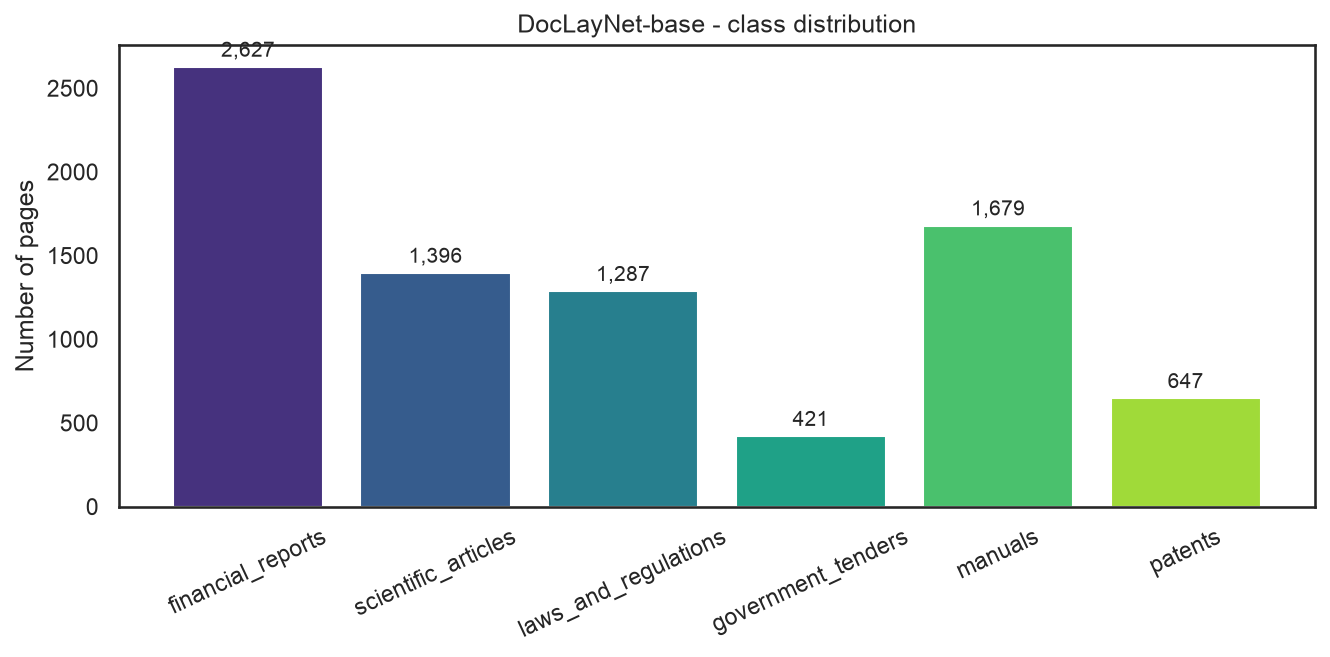
\includegraphics[width=0.85\linewidth]{figures/f1_class_distribution.png}
\caption{Class distribution of the DocLayNet-base dataset used in this study.
The six functional document types are strongly imbalanced, with
\texttt{financial\_reports} the largest and \texttt{government\_tenders} the
smallest class, which motivates class-weighted loss and augmentation.}
\label{fig:dist}
\end{figure}

\begin{figure}[!ht]
\centering
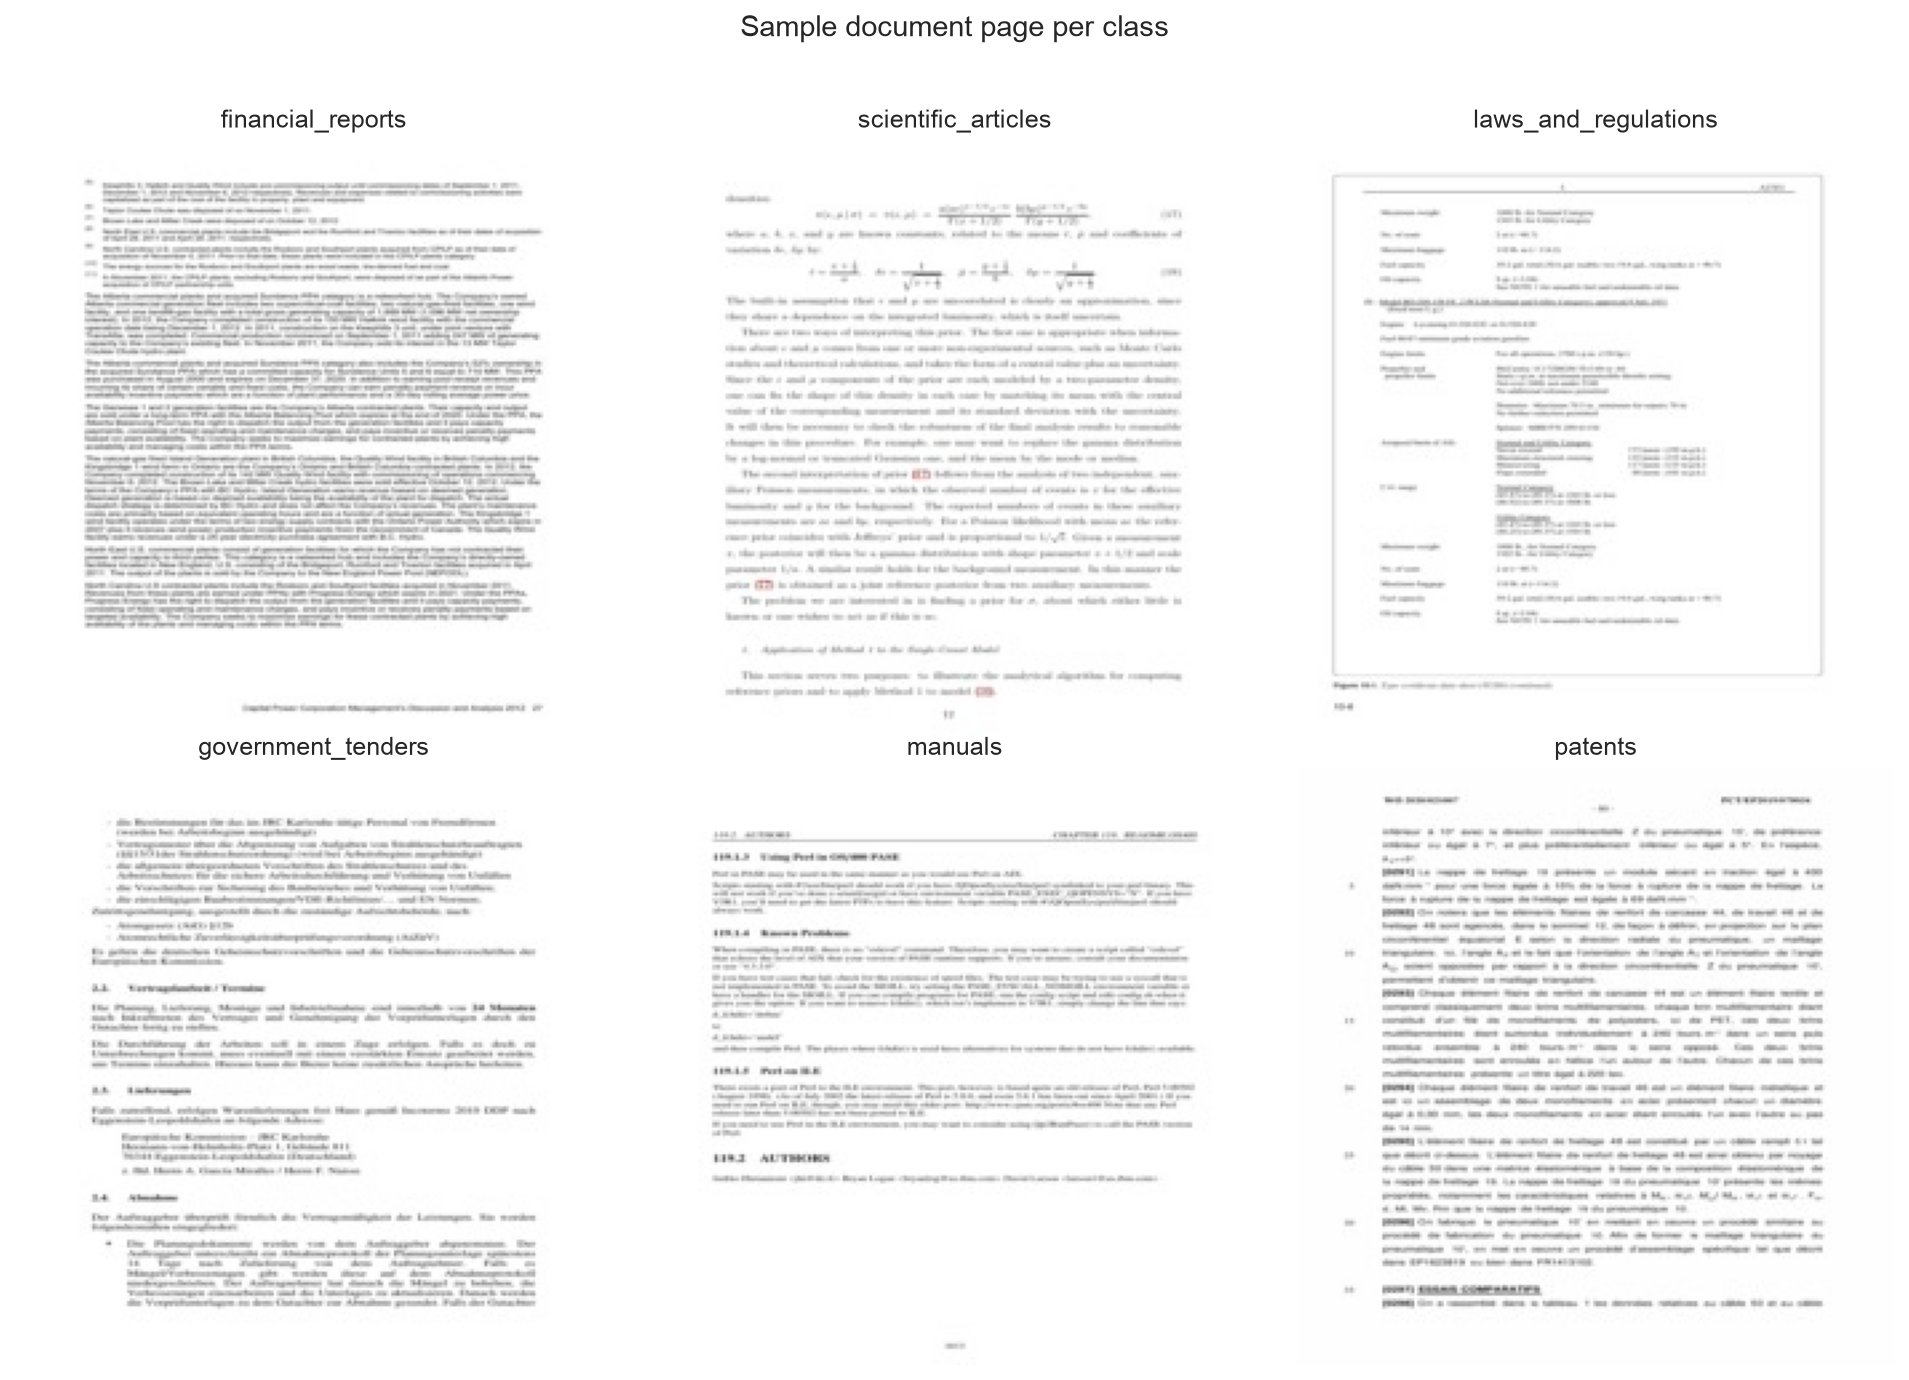
\includegraphics[width=0.95\linewidth]{figures/f2_sample_per_class.png}
\caption{One representative scanned page per class. The six categories differ in
masthead style, column structure, table density, and whitespace --- the visual
cues a layout-based CNN is expected to learn.}
\label{fig:samples}
\end{figure}

\subsection{Data Preparation}
\subsubsection{Data Splitting}
Pages are split with stratification into 70\% training, 15\% validation, and
15\% test, seeded for reproducibility, ensuring no page appears in more than one
split.
\subsubsection{Image Preprocessing}
Each page is converted to RGB and resized to $224\times224$ to match ResNet50's
input and remain tractable on a single GPU.
Pixels are normalised with ImageNet per-channel statistics for ResNet50 and
$[0,1]$ scaling for the custom CNN.
\subsubsection{Data Augmentation}
Training-time augmentation applies small random rotations ($\pm5^{\circ}$),
translations ($\pm5\%$), zoom ($\pm10\%$), and brightness shifts
($\pm15\%$)~\cite{shorten2019survey}; orientation-changing flips are avoided
because page orientation is informative.
\subsubsection{Class-Imbalance Handling}
Class-weighted categorical cross-entropy is used, with
$w_c = N/(C\cdot N_c)$ for class $c$, total samples $N$, and $C=6$ classes, so
minority classes contribute proportionally more to the loss.

\subsection{Model Development}
\subsubsection{Custom CNN Baseline}
The baseline accepts $224\times224\times3$ inputs and stacks four convolutional
blocks with 32, 64, 128, and 256 filters; each block applies a $3\times3$
convolution, batch normalisation~\cite{ioffe2015batch}, ReLU, and $2\times2$
max-pooling.
Global average pooling feeds a Dense(128)+ReLU layer with
Dropout(0.5)~\cite{srivastava2014dropout} and a Dense(6) softmax head
($\approx0.42$\,M parameters), trained from scratch.
\subsubsection{Transfer-Learning Model: ResNet50}
ResNet50~\cite{he2016deep} with ImageNet weights is used with a custom head:
Global Average Pooling, Dense(256)+ReLU, Dropout(0.4), and Dense(6) softmax.
\subsubsection{Feature Extraction and Fine-Tuning Strategy}
Training is two-stage: Stage~A freezes the backbone and trains only the head
(10 epochs, lr~$=10^{-3}$); Stage~B unfreezes the final residual block
(\texttt{conv5\_*}) and fine-tunes at lr~$=10^{-5}$ for 20 epochs, refining
pretrained features without catastrophic forgetting.

\subsection{Training Procedure}
The loss is class-weighted categorical cross-entropy, optimised with
Adam~\cite{kingma2014adam}, batch size 32, with early stopping on validation
accuracy.
Hyperparameters are summarised in Table~\ref{tab:hparams}.

\begin{table}[!ht]
\centering
\caption{Training configuration shared across both models, with the two-stage
schedule specific to the ResNet50 transfer-learning model.}
\label{tab:hparams}
\begin{tabular}{ll}
\toprule
\textbf{Setting} & \textbf{Value} \\
\midrule
Input size & $224\times224\times3$ \\
Optimiser & Adam \\
Batch size & 32 \\
Custom CNN learning rate & $1\times10^{-3}$ \\
ResNet50 Stage A (head) & 10 epochs, lr $1\times10^{-3}$ \\
ResNet50 Stage B (fine-tune \texttt{conv5\_*}) & 20 epochs, lr $1\times10^{-5}$ \\
Loss & Class-weighted categorical cross-entropy \\
Regularisation & Dropout (0.4--0.5), early stopping \\
Split & Stratified 70/15/15 \\
Random seed & 42 \\
\bottomrule
\end{tabular}
\end{table}

\subsection{Evaluation Framework}
Accuracy is the fraction of pages whose predicted type matches the true type:
\begin{equation}
\text{Accuracy} = \frac{\text{correctly classified pages}}{\text{total pages}}.
\label{eq:acc}
\end{equation}
Per class $c$, precision and recall are
\begin{equation}
P_c = \frac{TP_c}{TP_c+FP_c}, \qquad R_c = \frac{TP_c}{TP_c+FN_c},
\label{eq:pr}
\end{equation}
where $TP_c$, $FP_c$, and $FN_c$ are the pages correctly assigned to $c$,
wrongly assigned to $c$, and belonging to $c$ but missed.
The macro-F1 averages the per-class F1 equally across the six classes:
\begin{equation}
\text{macro-F1} = \frac{1}{C}\sum_{c=1}^{C}\frac{2P_cR_c}{P_c+R_c}.
\label{eq:f1}
\end{equation}
We additionally report one-vs-rest ROC curves with per-class and macro AUC,
confusion matrices, trainable-parameter counts, and a phone-camera robustness
delta.

\subsection{Explainable AI and Robustness}
Grad-CAM~\cite{selvaraju2017grad} is computed on the final convolutional layer of
ResNet50 to visualise the page regions driving each prediction.
Robustness is measured on a phone-camera-simulated test set (perspective warp,
JPEG compression, Gaussian blur, brightness shift), reporting the macro-F1 drop
versus clean images.
% TODO(student): SHAP is required by the template's XAI section but is not yet
% implemented; either add it or keep it scoped to future work.

\subsection{Software, Hardware, and Reproducibility}
The notebook runs on a Kaggle GPU (T4) with TensorFlow/Keras; seeds are fixed for
\texttt{numpy}, \texttt{random}, \texttt{tensorflow}, and \texttt{langdetect}.
Code, the trained model, figures, and the deployed service are public (see
Section~\ref{sec:links}).

%==================================================================
\section{Results}\label{sec:results}

\subsection{Dataset and Preprocessing Results (RQ1)}
After parsing, 8{,}057 usable pages were retained across the six classes with the
imbalance shown in Figure~\ref{fig:dist} and per-class samples in
Figure~\ref{fig:samples}, and split 70/15/15.

\subsection{Overall Model Performance (RQ2)}
Table~\ref{tab:compare} and Figure~\ref{fig:compare} report test-set
performance.
ResNet50 attains 0.761 accuracy, 0.724 macro-F1, and 0.956 macro-AUC, while the
custom CNN reaches only 0.326 accuracy and 0.082 macro-F1 at 0.479 macro-AUC.
The numerically strongest model is ResNet50 by a wide margin.

\begin{table}[!ht]
\centering
\caption{Test-set comparison of the custom CNN and the ResNet50 transfer-learning
model on the DocLayNet-base hold-out split, reporting parameter count and
macro-averaged metrics. ResNet50 dominates on every metric.}
\label{tab:compare}
\begin{tabular}{lrrrrrr}
\toprule
Model & Params & Accuracy & Macro-P & Macro-R & Macro-F1 & Macro-AUC \\
\midrule
Custom CNN & 0.42\,M & 0.326 & 0.054 & 0.167 & 0.082 & 0.479 \\
ResNet50   & 24.1\,M & \textbf{0.761} & \textbf{0.719} & \textbf{0.780} & \textbf{0.724} & \textbf{0.956} \\
\bottomrule
\end{tabular}
\end{table}

\begin{figure}[!ht]
\centering
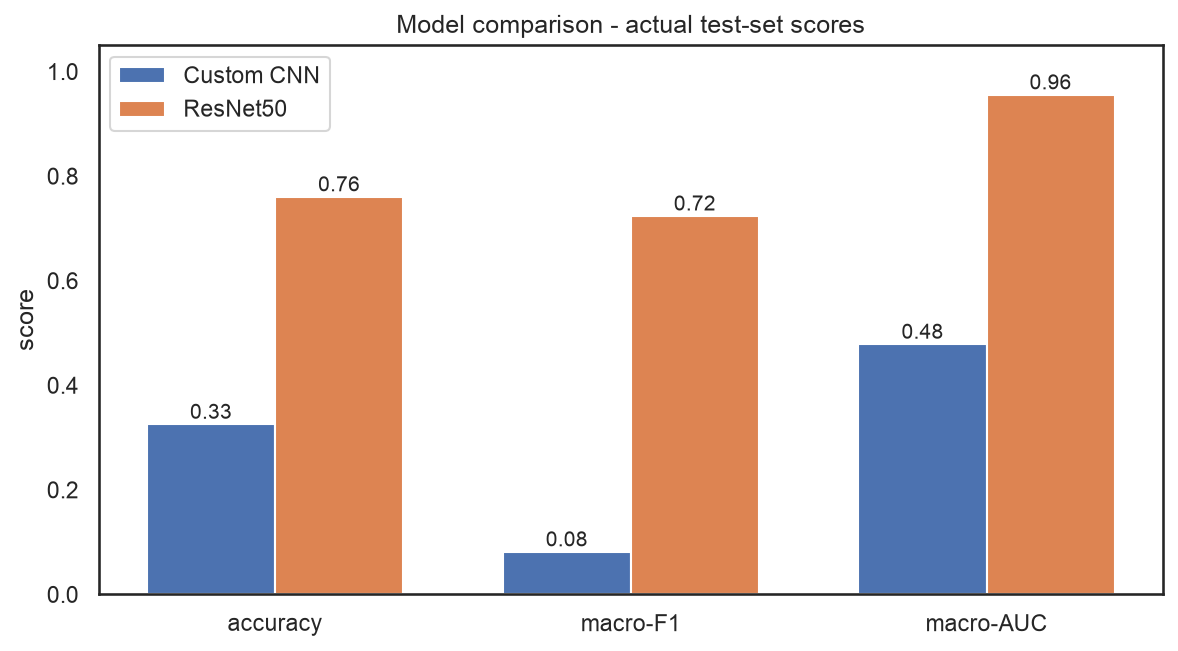
\includegraphics[width=0.7\linewidth]{figures/f9_model_comparison.png}
\caption{Accuracy, macro-F1, and macro-AUC for the custom CNN versus ResNet50 on
the test set. Transfer learning yields a large, consistent improvement across all
three metrics.}
\label{fig:compare}
\end{figure}

\subsection{Class-Level Performance (RQ3)}
Figure~\ref{fig:resnet} shows the ResNet50 confusion matrix and ROC curves, and
Figure~\ref{fig:cnn} the custom CNN.
ResNet50 is strong across classes, with residual confusion concentrated in
\texttt{scientific\_articles}, its lowest per-class AUC and the class most often
confused with text-dense financial and patent pages.
The custom CNN collapses toward the majority class, consistent with its
near-chance macro-AUC.

\begin{figure}[!ht]
\centering
\begin{subfigure}{0.49\linewidth}\centering
  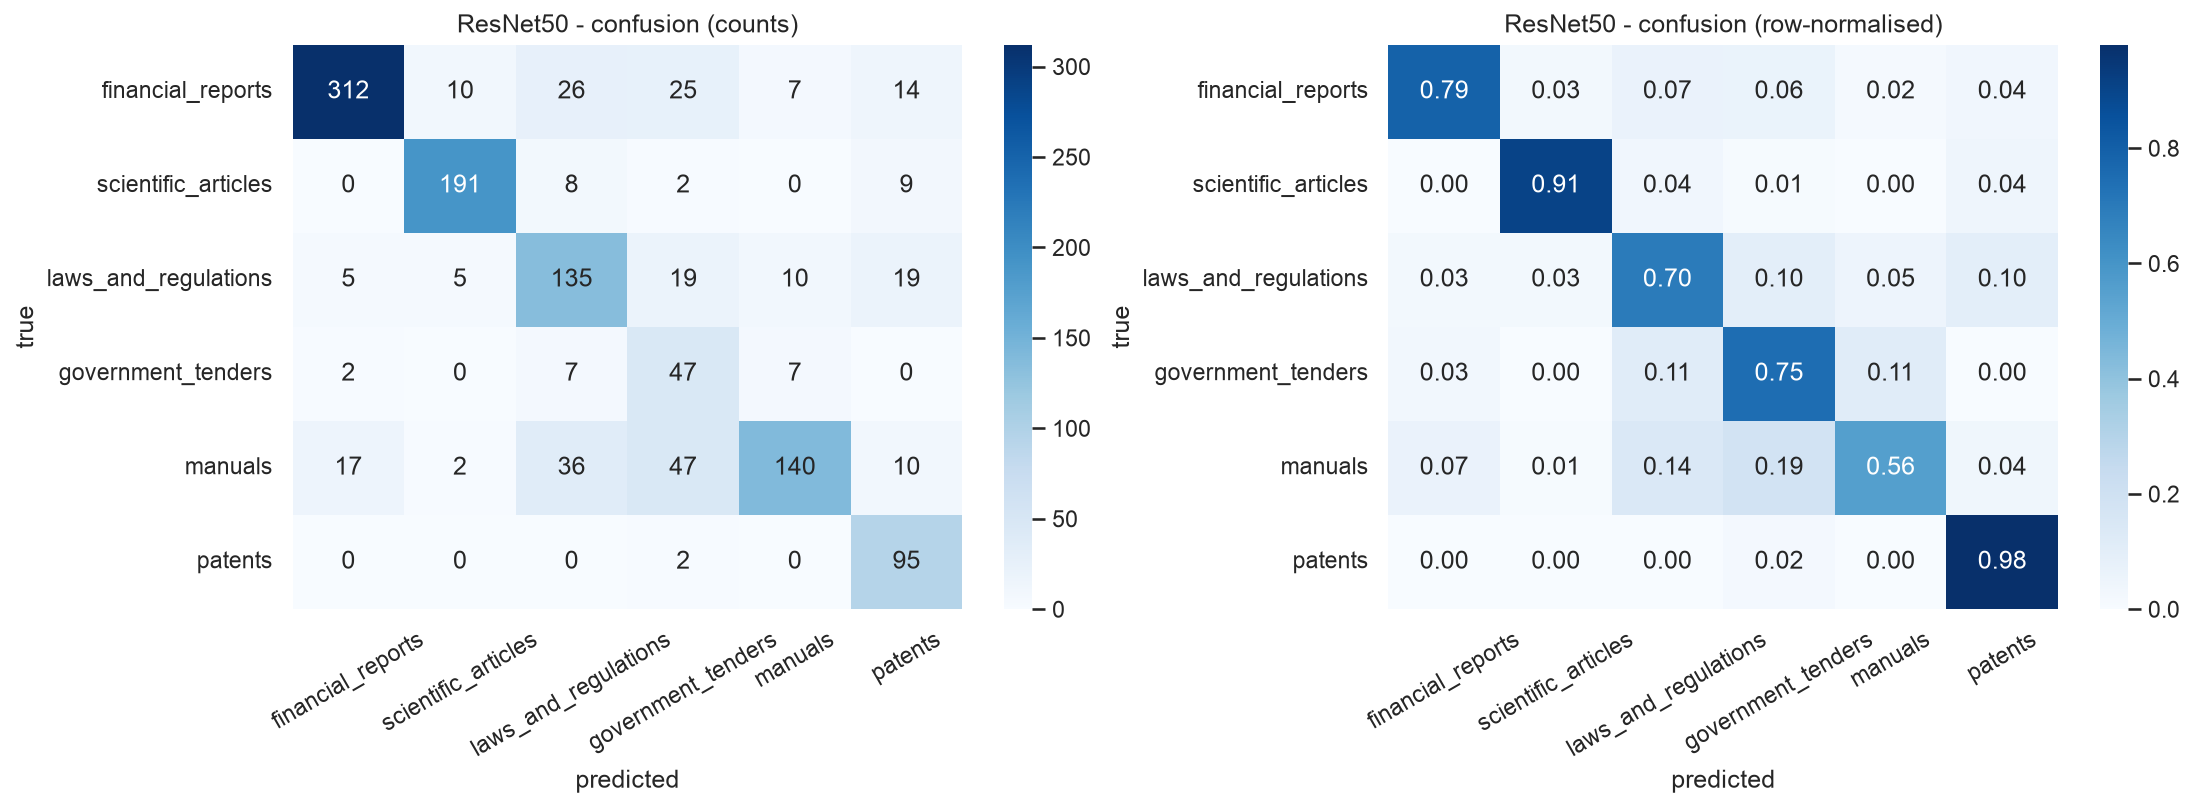
\includegraphics[width=\linewidth]{figures/f7_resnet50_confusion.png}
  \caption{ResNet50 confusion matrix.}
\end{subfigure}\hfill
\begin{subfigure}{0.49\linewidth}\centering
  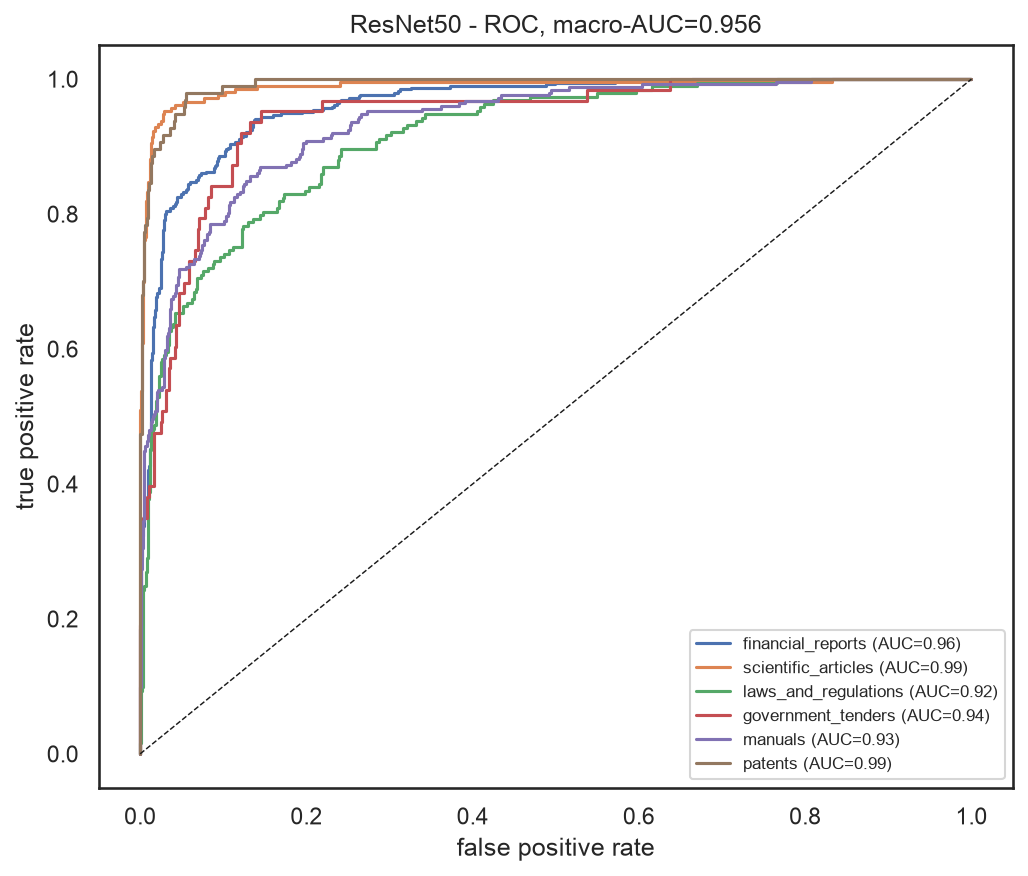
\includegraphics[width=\linewidth]{figures/f8_resnet50_roc.png}
  \caption{ResNet50 ROC curves (macro-AUC 0.956).}
\end{subfigure}
\caption{Per-class behaviour of the ResNet50 model: counts/row-normalised
confusion matrix (left) and one-vs-rest ROC curves with per-class AUC (right).
Errors concentrate in \texttt{scientific\_articles}.}
\label{fig:resnet}
\end{figure}

\begin{figure}[!ht]
\centering
\begin{subfigure}{0.49\linewidth}\centering
  
\includegraphics[width=\linewidth]{figures/f5_custom_cnn_confusion.png}
  \caption{Custom CNN confusion matrix.}
\end{subfigure}\hfill
\begin{subfigure}{0.49\linewidth}\centering
  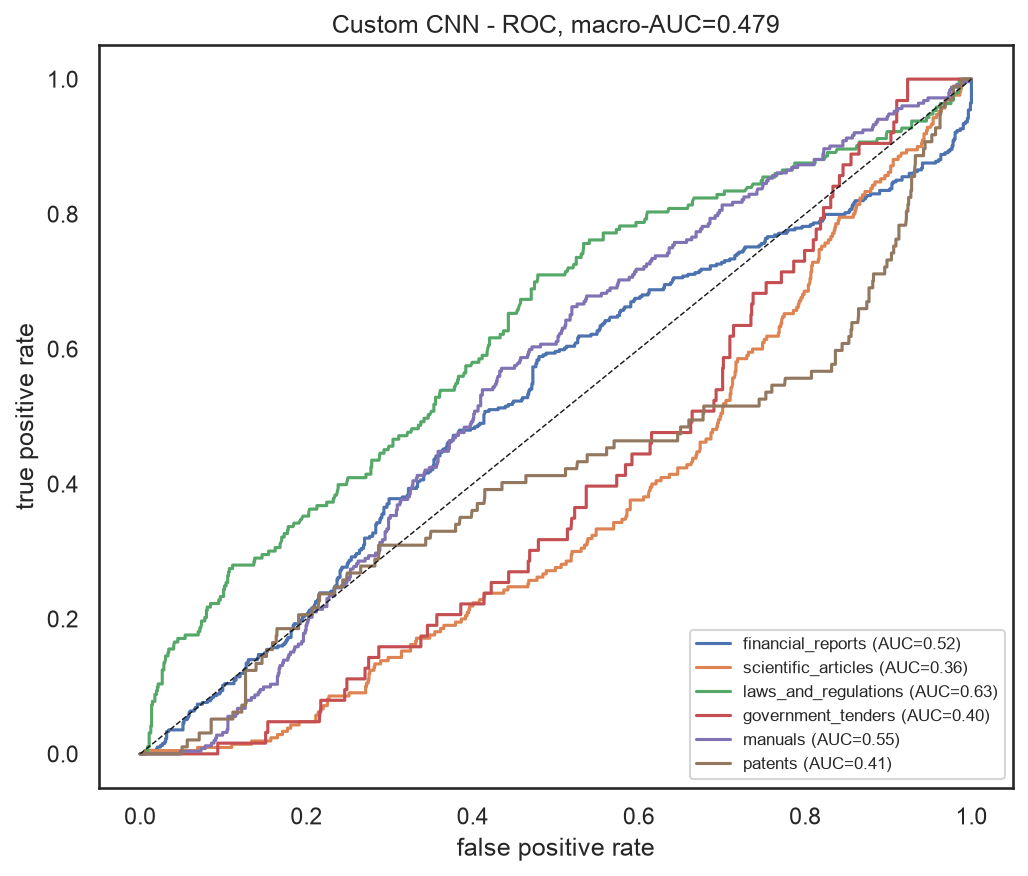
\includegraphics[width=\linewidth]{figures/f6_custom_cnn_roc.png}
  \caption{Custom CNN ROC curves.}
\end{subfigure}
\caption{The from-scratch custom CNN collapses toward the majority class,
producing near-diagonal-free confusion and near-chance ROC behaviour.}
\label{fig:cnn}
\end{figure}

\subsection{Explainable AI Results (RQ4)}
Figure~\ref{fig:gradcam} shows Grad-CAM overlays for ResNet50, one example page
per class.
The activation consistently falls on mastheads, headers, and structural regions
rather than arbitrary body text, supporting the layout-based hypothesis.
% TODO(student): SHAP results are required by the template; add when implemented.

\begin{figure}[!ht]
\centering
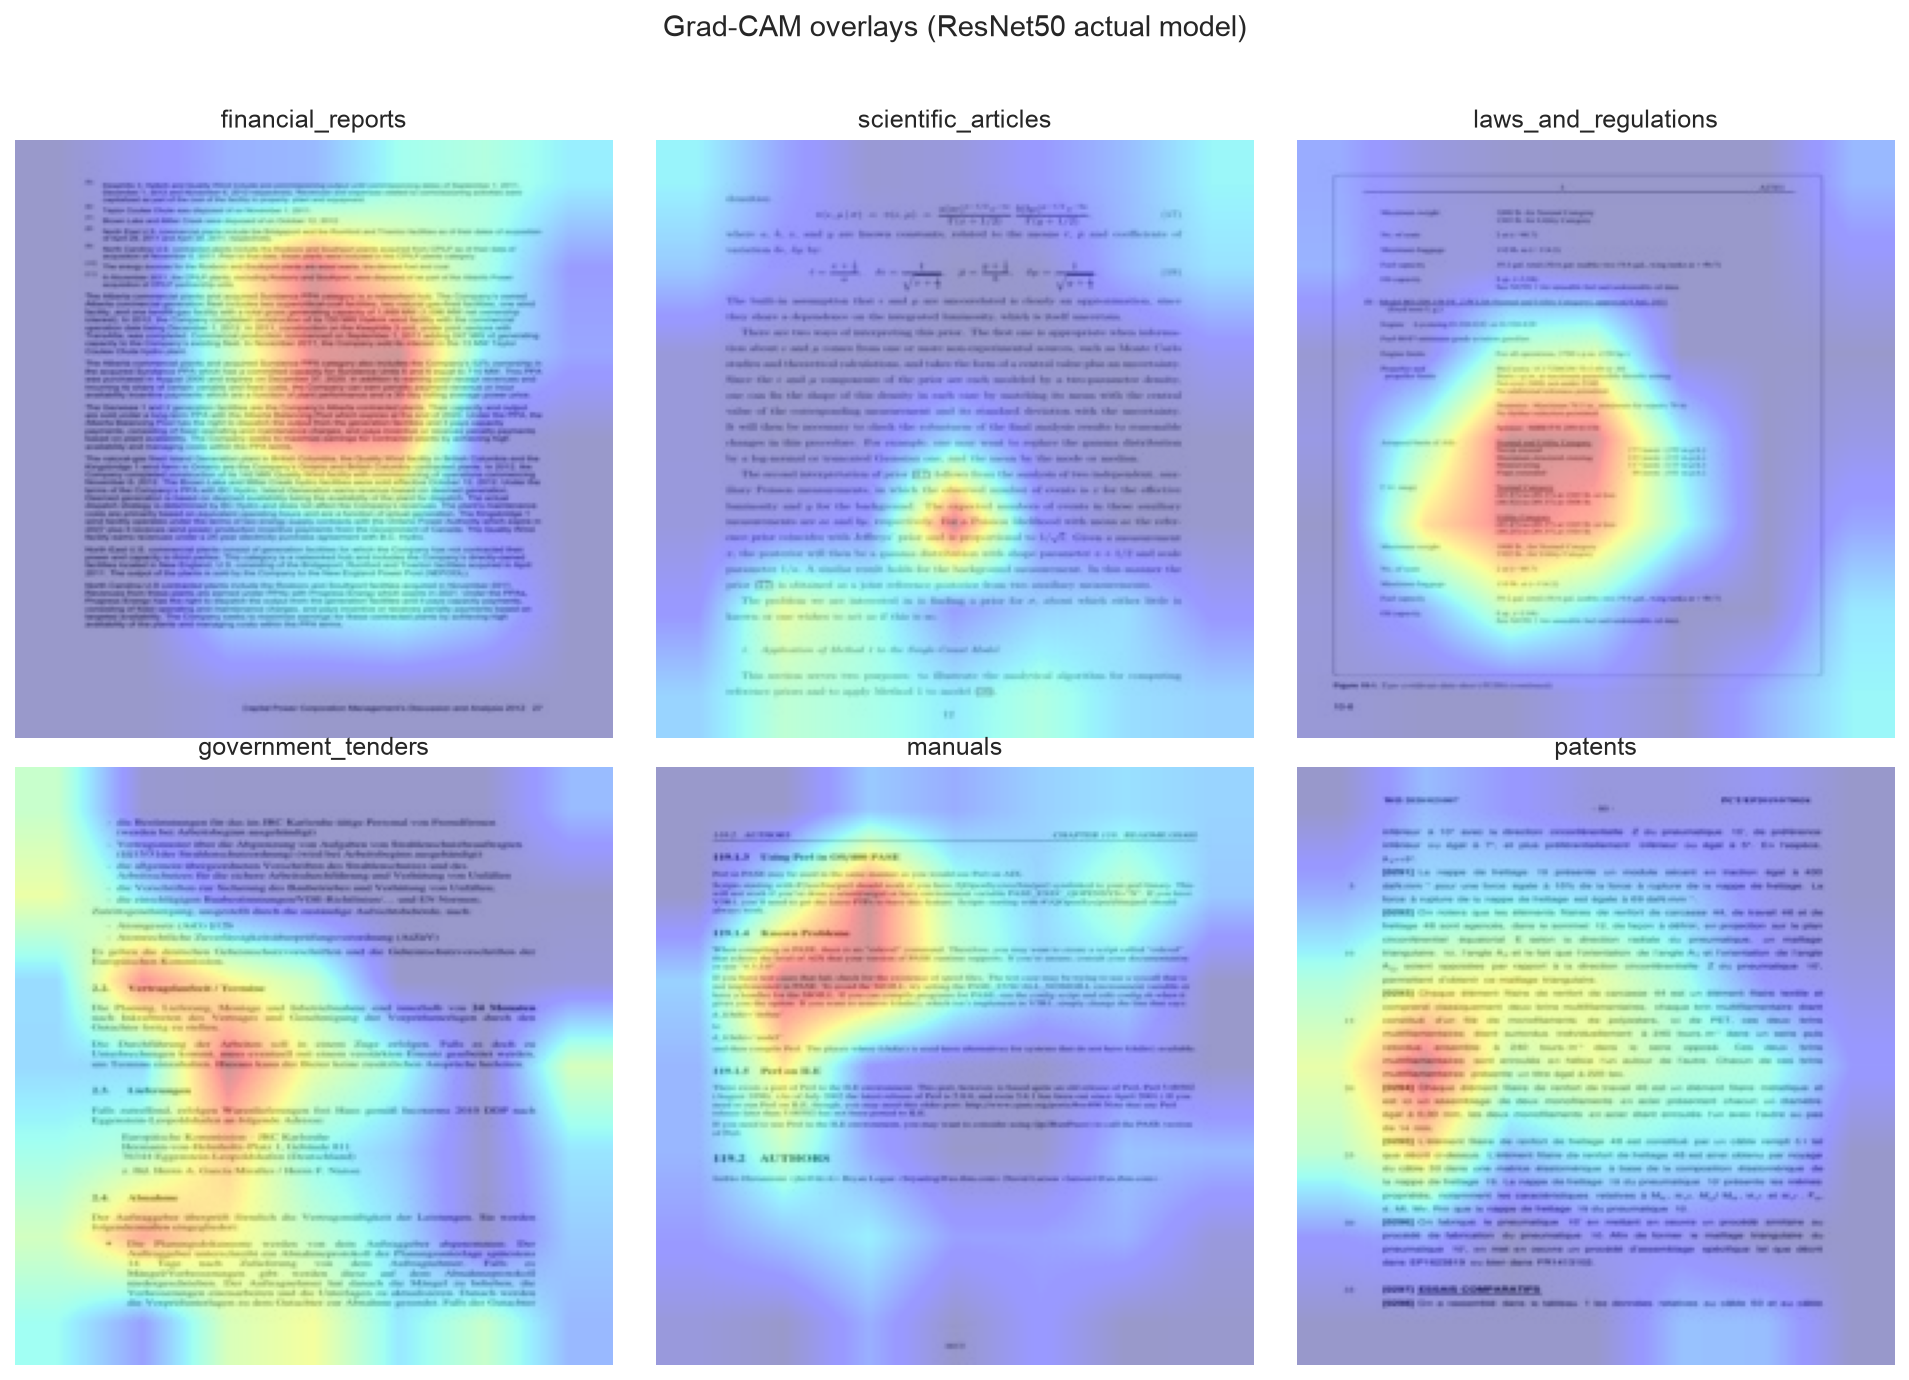
\includegraphics[width=0.95\linewidth]{figures/f10_gradcam.png}
\caption{Grad-CAM overlays for the ResNet50 model, one representative page per
class. Warm regions indicate the page areas most responsible for the predicted
type; attention concentrates on mastheads and structural layout regions.}
\label{fig:gradcam}
\end{figure}

\subsection{Robustness, Efficiency, and Deployment (RQ5)}
Figure~\ref{fig:robust} compares clean and phone-camera-simulated macro-F1.
ResNet50 degrades gracefully, from 0.724 to 0.606 ($-0.118$), while the collapsed
custom CNN shows no change.
At 24.1\,M parameters, ResNet50 is efficient enough for CPU deployment: it is
converted to TensorFlow Lite and served with a lightweight runtime in a
512\,MB-class container, with inference offloaded to a worker thread so the
service stays responsive.

\begin{figure}[!ht]
\centering

\includegraphics[width=0.6\linewidth]{figures/f11_robustness.png}
\caption{Robustness of both models: clean test macro-F1 versus
phone-camera-simulated macro-F1. ResNet50 loses about 0.118 macro-F1 but remains
usable; the collapsed custom CNN is unaffected because it already predicts a
single class.}
\label{fig:robust}
\end{figure}

\subsection{Summary of Research-Question Findings}
RQ1: layout-only classification is feasible (ResNet50 0.761 accuracy).
RQ2: ResNet50 clearly wins over the custom CNN.
RQ3: errors concentrate in the visually confusable \texttt{scientific\_articles}.
RQ4: Grad-CAM confirms attention on meaningful regions.
RQ5: the model is robust and deployable.

%==================================================================
\section{Discussion}\label{sec:discussion}

\subsection{Comparative Performance of CNN Models (RQ1, RQ2)}
The central finding is that transfer learning is not merely better but necessary
on this small, imbalanced dataset.
ImageNet features give ResNet50 the low-level priors a $0.42$\,M-parameter
network cannot learn from scratch, and the from-scratch CNN never escapes
near-chance macro-AUC.
This is consistent with prior document-image findings that pretraining
dominates on limited data~\cite{afzal2017cutting,weiss2016survey}.

\subsection{Class-Level Reliability and Error Patterns (RQ3)}
Errors concentrate in \texttt{scientific\_articles}, which is visually similar to
text-dense financial and patent pages, lowering its per-class AUC.
Class imbalance amplifies this, since minority and visually ambiguous classes are
hardest, and the class-weighted loss only partly compensates.

\subsection{Interpretation of Grad-CAM (RQ4)}
Grad-CAM indicates the model attends to mastheads and structural regions rather
than background artefacts, increasing trust in the predictions.
However, heatmaps are not proof of causal reasoning, and adding SHAP would
strengthen the explainability claim.

\subsection{Efficiency and Practical Deployment (RQ5)}
The accuracy-efficiency trade-off favours ResNet50: it is accurate and small
enough to run on CPU once converted to TensorFlow Lite, enabling a free-tier
web deployment with worker-thread inference.
This demonstrates practical feasibility for document-routing assistants, with
human oversight for low-confidence cases.

\subsection{Limitations}
The study uses a single dataset and a single stratified split, evaluates on the
all-languages DocLayNet-base rather than the strictly German-filtered subset
(re-run pending), implements Grad-CAM but not SHAP, and does not perform external
validation or statistical significance testing.

\subsection{Future Research Directions}
Future work includes completing the German-filtered re-training with the yield
report, adding SHAP and statistical comparison, targeting the weak
\texttt{scientific\_articles} class with focused augmentation, exploring
EfficientNet/DenseNet backbones, and adding a confidence/out-of-distribution gate
for non-target uploads.

%==================================================================
\section{Conclusion}\label{sec:conclusion}
This study built and evaluated an explainable CNN framework that classifies
scanned German document pages into six DocLayNet types from visual layout alone.
A two-stage fine-tuned ResNet50 reached 0.761 accuracy, 0.724 macro-F1, and
0.956 macro-AUC, decisively outperforming a from-scratch custom CNN that
collapsed to near-chance.
Grad-CAM confirmed that the model attends to mastheads and structural regions,
and the model degraded by only about 0.118 macro-F1 under phone-camera
simulation while remaining small enough to deploy as a public web service.
The principal limitation is reliance on a single dataset without SHAP or external
validation, and the immediate future direction is completing the strictly
German-filtered re-training.

\section*{Repository and Notebook Links}\label{sec:links}
\begin{itemize}
\item Live demo: \url{https://document-type-classification-framework.onrender.com}
\item GitHub: \url{https://github.com/ashok-cse/Document-Type-Classification-Framework}
\item Kaggle: \url{https://www.kaggle.com/code/ashokkrcse/german-document-type-classification-with-cnns}
\end{itemize}

\section*{Declarations}
The author used a generative AI tool to improve the language and clarity of the
manuscript.
The author reviewed and edited all content and takes full responsibility for the
final version.

% DO NOT REMOVE THESE LINES
\bibliographystyle{elsarticle-num}
\bibliography{Bibliography}

\end{document}
